

\begin{tikzpicture}[]


%%% DEFINITIONS %%%%%%%%%%%%%%%%%%%%%%%%%%%%%%%%%%%%%%%%%%%%%%%%%%%%%%%%%%%%%


% https://associatie.kuleuven.be/huisstijl/kleuren
\definecolor{blue1}{RGB}{82,189,236}
\definecolor{blue2}{RGB}{0,64,122}
\definecolor{blue3}{RGB}{31,171,231}
\definecolor{blue4}{RGB}{29,141,176}
\definecolor{blue5}{RGB}{17,110,138}
\definecolor{orange1}{RGB}{221,138,46}


\def\ThPoolCenterOneX{-2}
\def\ThPoolCenterOneY{0}

\def\ThPoolCenterTwoX{2}
\def\ThPoolCenterTwoY{0}


%%% DRAWING %%%%%%%%%%%%%%%%%%%%%%%%%%%%%%%%%%%%%%%%%%%%%%%%%%%%%%%%%%%%%%%%%

\node at (0, 3) {\LARGE Process};

\draw [black] (0,0) ellipse (8 and 4);


\node [align=center] at (-10, 2) {\large CPU \\ \large thread pool};
\node [align=center] at (+10, 2) {\large GPU \\ \large thread pool};

\draw (-8.25,1.7) -- (-6,1);
\draw (8.25,1.7) -- (6,1);

\filldraw [blue1, opacity=0.1] (\ThPoolCenterOneX-2,\ThPoolCenterOneY) circle (2.8);
\filldraw [blue2, opacity=0.1] (\ThPoolCenterTwoX+1.8,\ThPoolCenterOneY) circle (2.8);
\draw [blue1] (\ThPoolCenterOneX-2,\ThPoolCenterOneY) circle (2.8);
\draw [blue2] (\ThPoolCenterTwoX+1.8,\ThPoolCenterOneY) circle (2.8);


\foreach \x in {1,...,3} {
    \node[inner sep=0pt] at (\ThPoolCenterOneX-\x, 1.5){
\includegraphics[width=1em]{figure/session-1/thread-small.png}};
}
\foreach \x in {0,...,4} {
    \node[inner sep=0pt] at (\ThPoolCenterOneX-\x, 0){
\includegraphics[width=1em]{figure/session-1/thread-small.png}};
}
\foreach \x in {1,...,3} {
    \node[inner sep=0pt] at (\ThPoolCenterOneX-\x, -1.5){
\includegraphics[width=1em]{figure/session-1/thread-small.png}};
}


\foreach \x in {1,...,6} {
    \node[inner sep=0pt] at (\ThPoolCenterTwoX+\x/2, 1.5){
\includegraphics[width=1em]{figure/session-1/thread-small.png}};
}
\foreach \x in {-1,...,8} {
    \node[inner sep=0pt] at (\ThPoolCenterTwoX+\x/2, 0){
\includegraphics[width=1em]{figure/session-1/thread-small.png}};
}
\foreach \x in {1,...,6} {
    \node[inner sep=0pt] at (\ThPoolCenterTwoX+\x/2, -1.5){
\includegraphics[width=1em]{figure/session-1/thread-small.png}};
}


\draw [->] (-8.5,0) to [out=180,in=90] (-10,-2.5);
\draw [->] (+8.5,0) to [out=0,in=90] (+10,-2.5);

\node [align=center] at (-11.5, -0.5) {Map threads \\ to CPU cores};
\node [align=center] at (+11.5, -0.5) {Map threads \\ to GPU cores};

\node[inner sep=0pt] at (-10, -5){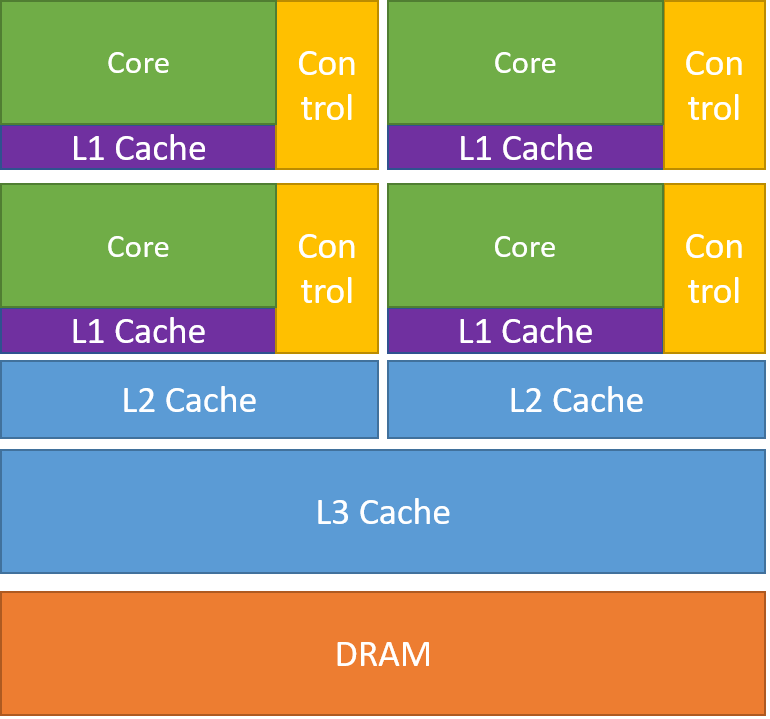
\includegraphics[width=10em]{figure/session-1/cpu-architecture.png}};

\node[inner sep=0pt] at (+10, -5){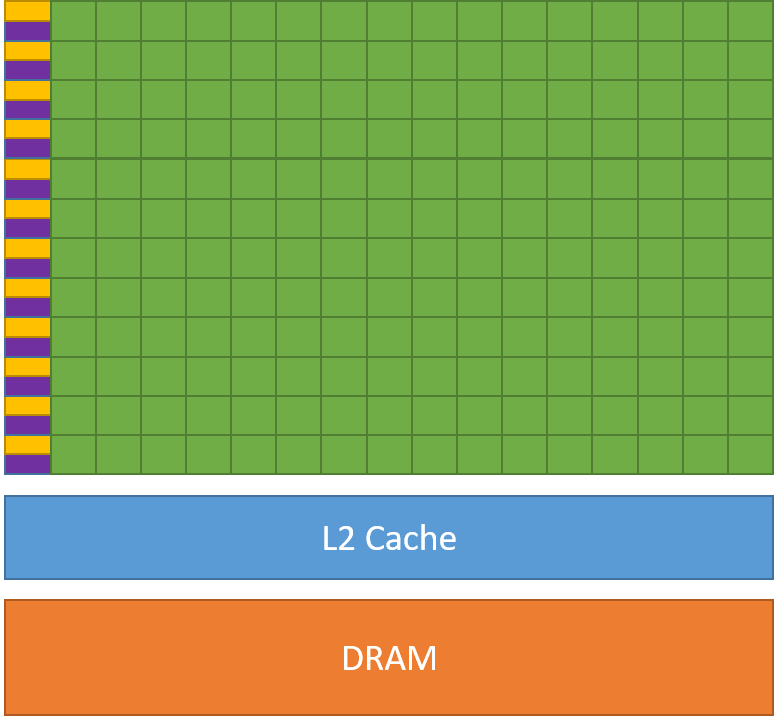
\includegraphics[width=10em]{figure/session-1/gpu-architecture.png}};



\end{tikzpicture}